% paper/manuscript/supplement.tex
% Supplementary material for the ShellForm manuscript (Computers & Structures).
% S1 literature search protocol (paper/13_literature_search.md),
% S2 Fig. S1 (figures/figS1_verification.pdf), S3 pre-registration amendments
% (docs/preregistration.md, summarised), S4 Table S1 (paper/tables/tableS1_all_designs.md).
% Build: latexmk -pdf supplement.tex

\documentclass[11pt,a4paper]{article}
\usepackage[T1]{fontenc}
\usepackage[utf8]{inputenc}
\usepackage{lmodern}
\usepackage[margin=22mm]{geometry}
\usepackage{amsmath,amssymb}
\usepackage{graphicx,booktabs,array,longtable,xcolor}
\usepackage[hidelinks]{hyperref}
\usepackage{url}
\graphicspath{{../../figures/}}
\renewcommand{\thefigure}{S\arabic{figure}}
\renewcommand{\thetable}{S\arabic{table}}
\renewcommand{\thesection}{S\arabic{section}}
\definecolor{markcol}{HTML}{B4462B}
\newcommand{\chk}{\textsuperscript{\textcolor{markcol}{\sffamily\scriptsize[check]}}}

\title{Supplementary material\\[1ex]\large Does seismic-aware form-finding lower the embodied carbon of reinforced concrete shells? A pre-registered comparison of 168 sized designs}
\author{Syed Nafiz Reja Hasib}
\date{}

\begin{document}
\maketitle

\section{Literature search protocol}

The gap statement of Section~1 rests on a documented search, run on 13 November 2026 in OpenAlex (about 250 million records, open access and paywalled). The search window was 2015--2026, to include the work of Michiels and Adriaenssens (2017--2019); the gap claim rests on papers from 2020--2026. A paper was included if it studies (a) form-finding or shape design of shells or arches under lateral or seismic load, (b) the embodied carbon of concrete shells or shell floors, or (c) the seismic response of concrete shells. Retrofit, frames, walls, tanks, piles and masonry infill were excluded.

\begin{table}[h]
\centering\small
\caption{Search queries, screening and inclusion.}
\begin{tabular}{llrrr}
\toprule
Query & Words & From & Screened & Included\\
\midrule
Q1 & form finding shell structures seismic lateral loading & 2015 & top 20 & 5\\
Q2 & embodied carbon concrete shell structures form-finding & 2018 & top 20 & 6\\
Q3 & thin concrete shell roof seismic behaviour reinforced concrete earthquake & 2015 & top 20 & 1\\
Q4 & earthquake response of thin reinforced concrete shell roofs stiffness low mass parametric & 2016 & top 10 & 2\\
Q5 & concrete shell form finding optimisation material reduction buckling governs thickness & 2018 & top 10 & 1\\
Q6 & embodied carbon seismic design shell form-found compression-only lateral load material efficiency & 2019 & top 10 & 0\\
\bottomrule
\end{tabular}
\end{table}

Q6 found no paper that reports the embodied carbon of seismic-aware form-finding. Forward citation searching from Michiels and Adriaenssens (2017, 2018) is still to be done\chk. The full log, with the 15 included papers, is \texttt{paper/13\_literature\_search.md} in the repository.

\section{Verification of the analysis chain}

\begin{figure}[h]
\centering
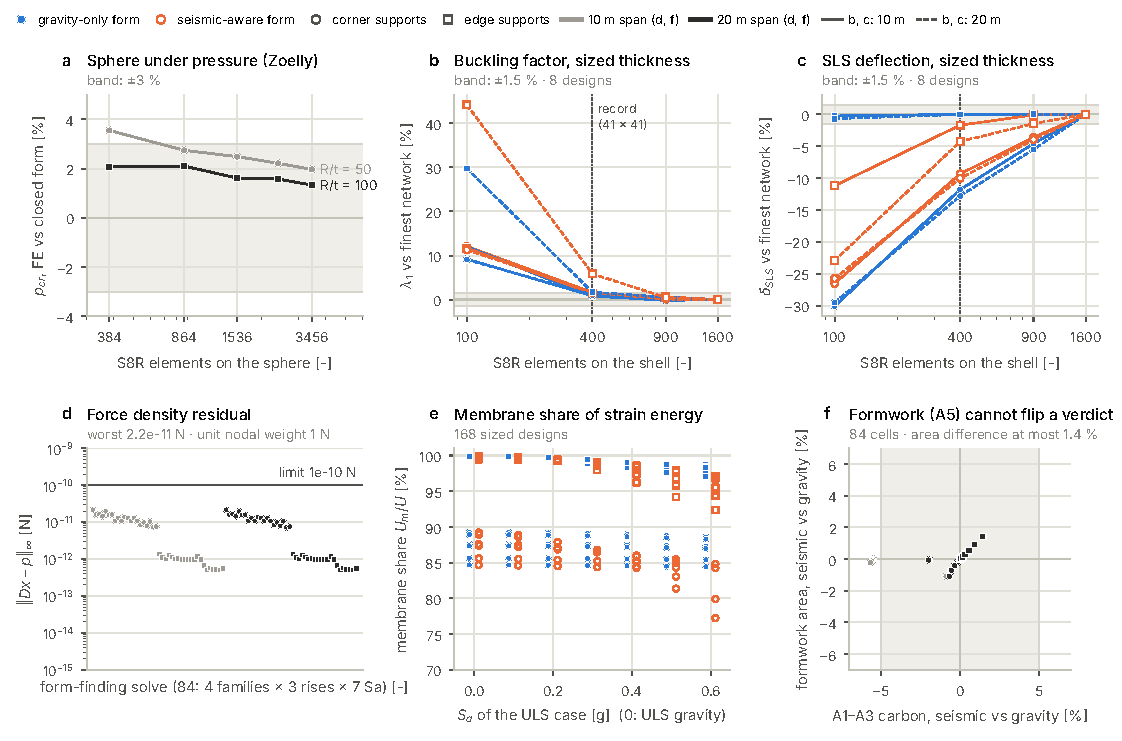
\includegraphics[width=\textwidth]{figS1_verification.pdf}
\caption{Verification checks V1--V5, run after the freeze (Section~3.6 of the paper): (a) sphere buckling against the classical value; (b) first buckling factor and (c) SLS deflection under mesh refinement from 21 to 81 nodes per side; (d) residual of the assembled force density system; (e) membrane share of strain energy; (f) soffit area difference against carbon difference (formwork bound).}
\end{figure}

\section{Pre-registration amendments}

The pre-registration of 28--30 October 2026 and every dated amendment are in \texttt{docs/preregistration.md}. Each amendment states whether it was written before or after the results it affects. In summary:

\begin{longtable}{p{0.16\textwidth}p{0.20\textwidth}p{0.56\textwidth}}
\toprule
Date (2026) & Timing & Change\\
\midrule
\endhead
30 Oct & before any run & Seismic-aware strategy defined (four directions, envelope check); own 3D solver; ICE replaced by a $\pm$25\,\% factor band; thresholds set ($\lambda$ 5, with 3 and 8; $L/300$; 50~mm; 5~mm steps; 5\,\% decision band). Midrange instead of mean of the four thrust surfaces.\\
31 Oct & before any design-space run & Corner-supported free edges drawn in by $0.10L$ (D3-1); own S8R deck, to be cross-checked against ShellBench's wrapper.\\
1 Nov & before the first sizing run & Seismic case in $+x$ only (symmetry); corner zones of $0.2L$ out of the compression check; characteristic deflection combination; bisection sizing.\\
1 Nov & after the 84 designs & Poisson's ratio read in place from ShellBench (value unchanged); loads per plan area recorded (D4-5); code basis for roof live load added. No thickness changed.\\
2 Nov & before the 84-design run & Steel rule (two directions, EN 1992-1-1 Annex F, no biaxial relief), minimum ratio in both directions, support-zone thickening, net steel.\\
3 Nov & after results; fix before the 20~m run & Carbon per m$^2$ of plan area for corner-supported shells (code followed the stated rule).\\
4 Nov & just after the S4 run & S4 fallback: closed-form lean of a parabolic arch (published arch not available).\\
6 Nov & during the sensitivity runs & How the three sensitivity runs were run (all 168 designs).\\
7 Nov & before the corrected runs & Pin moved to ShellBench v0.2.0 (0 mismatches); four buckling factors requested (D10-1).\\
8 Nov & citation only & EN 1992-1-1 Annex F read in full.\\
9 Nov & before the freeze run & Freeze one day early; pin ShellBench v0.3.0.\\
9 Nov & after the freeze & Presentation only (plotting style).\\
11 Nov & citation only & Buckling-threshold sources read (Dul\'acska and Koll\'ar 1995; ACI 318.2-14).\\
14 Nov & after the freeze, exploratory & Verification checks V1--V5 and Fig.~6; no result changed.\\
\bottomrule
\end{longtable}

\section{All 168 sized designs}

Table~S1 lists every sized design at the central carbon factors, with the low and high ends of the $\pm$25\,\% band. Design identifiers give span, supports, rise-to-span ratio, strategy and $S_a$ (g). The same values are in \texttt{paper/tables/tableS1\_all\_designs.csv}; the full record, with every check, is \texttt{results/batch\_all.csv} at tag \texttt{freeze-2026-11-09} (ShellBench v0.3.0).

\begin{center}
\scriptsize
\begin{longtable}{lrlrrrrrr}
\caption{All 168 sized designs.}\\
\toprule
design & t [mm] & governs & $\lambda$ [-] & T1 [s] & steel [kg] & carbon [kgCO$_2$e/m$^2$] & band low & band high \\
\midrule
\endfirsthead
\toprule
design & t [mm] & governs & $\lambda$ [-] & T1 [s] & steel [kg] & carbon [kgCO$_2$e/m$^2$] & band low & band high \\
\midrule
\endhead
\bottomrule
\endfoot
L10-corners-r0.10-gravity-sa0.0 & 105 & buckling & 5.05 & 0.184 & 275 & 45.5 & 34.1 & 56.9 \\
L10-corners-r0.10-gravity-sa0.1 & 105 & buckling & 5.05 & 0.184 & 275 & 45.5 & 34.1 & 56.9 \\
L10-corners-r0.10-gravity-sa0.2 & 105 & buckling & 5.05 & 0.184 & 275 & 45.5 & 34.1 & 56.9 \\
L10-corners-r0.10-gravity-sa0.3 & 105 & buckling & 5.05 & 0.184 & 275 & 45.5 & 34.1 & 56.9 \\
L10-corners-r0.10-gravity-sa0.4 & 105 & buckling & 5.05 & 0.184 & 275 & 45.5 & 34.1 & 56.9 \\
L10-corners-r0.10-gravity-sa0.5 & 105 & buckling & 5.05 & 0.184 & 275 & 45.5 & 34.1 & 56.9 \\
L10-corners-r0.10-gravity-sa0.6 & 105 & buckling & 5.05 & 0.184 & 275 & 45.5 & 34.1 & 56.9 \\
L10-corners-r0.10-seismic-sa0.0 & 105 & buckling & 5.05 & 0.184 & 275 & 45.5 & 34.1 & 56.9 \\
L10-corners-r0.10-seismic-sa0.1 & 105 & buckling & 5.06 & 0.184 & 275 & 45.5 & 34.1 & 56.9 \\
L10-corners-r0.10-seismic-sa0.2 & 105 & buckling & 5.07 & 0.184 & 275 & 45.5 & 34.1 & 56.9 \\
L10-corners-r0.10-seismic-sa0.3 & 105 & buckling & 5.08 & 0.184 & 275 & 45.5 & 34.1 & 56.9 \\
L10-corners-r0.10-seismic-sa0.4 & 105 & buckling & 5.09 & 0.183 & 275 & 45.5 & 34.1 & 56.9 \\
L10-corners-r0.10-seismic-sa0.5 & 105 & buckling & 5.10 & 0.183 & 275 & 45.5 & 34.1 & 56.9 \\
L10-corners-r0.10-seismic-sa0.6 & 105 & buckling & 5.10 & 0.182 & 275 & 45.5 & 34.1 & 56.9 \\
L10-corners-r0.15-gravity-sa0.0 & 90 & buckling & 5.60 & 0.159 & 238 & 39.8 & 29.9 & 49.8 \\
L10-corners-r0.15-gravity-sa0.1 & 90 & buckling & 5.60 & 0.159 & 238 & 39.8 & 29.9 & 49.8 \\
L10-corners-r0.15-gravity-sa0.2 & 90 & buckling & 5.60 & 0.159 & 238 & 39.8 & 29.9 & 49.8 \\
L10-corners-r0.15-gravity-sa0.3 & 90 & buckling & 5.60 & 0.159 & 238 & 39.8 & 29.9 & 49.8 \\
L10-corners-r0.15-gravity-sa0.4 & 90 & buckling & 5.60 & 0.159 & 238 & 39.8 & 29.9 & 49.8 \\
L10-corners-r0.15-gravity-sa0.5 & 90 & buckling & 5.60 & 0.159 & 238 & 39.8 & 29.9 & 49.8 \\
L10-corners-r0.15-gravity-sa0.6 & 90 & buckling & 5.60 & 0.159 & 238 & 39.8 & 29.9 & 49.8 \\
L10-corners-r0.15-seismic-sa0.0 & 90 & buckling & 5.60 & 0.159 & 238 & 39.8 & 29.9 & 49.8 \\
L10-corners-r0.15-seismic-sa0.1 & 85 & buckling & 5.02 & 0.165 & 225 & 37.7 & 28.3 & 47.1 \\
L10-corners-r0.15-seismic-sa0.2 & 85 & buckling & 5.04 & 0.164 & 225 & 37.7 & 28.2 & 47.1 \\
L10-corners-r0.15-seismic-sa0.3 & 85 & buckling & 5.05 & 0.164 & 225 & 37.6 & 28.2 & 47.1 \\
L10-corners-r0.15-seismic-sa0.4 & 85 & buckling & 5.05 & 0.165 & 225 & 37.6 & 28.2 & 47.0 \\
L10-corners-r0.15-seismic-sa0.5 & 85 & buckling & 5.03 & 0.167 & 224 & 37.6 & 28.2 & 47.0 \\
L10-corners-r0.15-seismic-sa0.6 & 90 & buckling & 5.63 & 0.161 & 237 & 39.7 & 29.8 & 49.7 \\
L10-corners-r0.20-gravity-sa0.0 & 75 & buckling & 5.41 & 0.165 & 204 & 34.3 & 25.7 & 42.9 \\
L10-corners-r0.20-gravity-sa0.1 & 75 & buckling & 5.41 & 0.165 & 204 & 34.3 & 25.7 & 42.9 \\
L10-corners-r0.20-gravity-sa0.2 & 75 & buckling & 5.41 & 0.165 & 204 & 34.3 & 25.7 & 42.9 \\
L10-corners-r0.20-gravity-sa0.3 & 75 & buckling & 5.41 & 0.165 & 204 & 34.3 & 25.7 & 42.9 \\
L10-corners-r0.20-gravity-sa0.4 & 75 & buckling & 5.41 & 0.165 & 204 & 34.3 & 25.7 & 42.9 \\
L10-corners-r0.20-gravity-sa0.5 & 75 & buckling & 5.41 & 0.165 & 204 & 34.3 & 25.7 & 42.9 \\
L10-corners-r0.20-gravity-sa0.6 & 75 & buckling & 5.41 & 0.165 & 204 & 34.3 & 25.7 & 42.9 \\
L10-corners-r0.20-seismic-sa0.0 & 75 & buckling & 5.41 & 0.165 & 204 & 34.3 & 25.7 & 42.9 \\
L10-corners-r0.20-seismic-sa0.1 & 75 & buckling & 5.50 & 0.164 & 204 & 34.3 & 25.7 & 42.9 \\
L10-corners-r0.20-seismic-sa0.2 & 75 & buckling & 5.54 & 0.164 & 204 & 34.3 & 25.7 & 42.9 \\
L10-corners-r0.20-seismic-sa0.3 & 75 & buckling & 5.52 & 0.167 & 203 & 34.3 & 25.7 & 42.8 \\
L10-corners-r0.20-seismic-sa0.4 & 75 & buckling & 5.45 & 0.170 & 203 & 34.2 & 25.6 & 42.7 \\
L10-corners-r0.20-seismic-sa0.5 & 75 & buckling & 5.34 & 0.175 & 202 & 34.1 & 25.6 & 42.6 \\
L10-corners-r0.20-seismic-sa0.6 & 75 & buckling & 5.26 & 0.180 & 203 & 34.0 & 25.5 & 42.5 \\
L10-edges-r0.10-gravity-sa0.0 & 50 & $t_{\mathrm{min}}$ & 67.93 & 0.045 & 173 & 21.6 & 16.2 & 27.0 \\
L10-edges-r0.10-gravity-sa0.1 & 50 & $t_{\mathrm{min}}$ & 67.93 & 0.045 & 173 & 21.6 & 16.2 & 27.0 \\
L10-edges-r0.10-gravity-sa0.2 & 50 & $t_{\mathrm{min}}$ & 67.93 & 0.045 & 173 & 21.6 & 16.2 & 27.0 \\
L10-edges-r0.10-gravity-sa0.3 & 50 & $t_{\mathrm{min}}$ & 67.93 & 0.045 & 173 & 21.6 & 16.2 & 27.0 \\
L10-edges-r0.10-gravity-sa0.4 & 50 & $t_{\mathrm{min}}$ & 67.93 & 0.045 & 173 & 21.6 & 16.2 & 27.0 \\
L10-edges-r0.10-gravity-sa0.5 & 50 & $t_{\mathrm{min}}$ & 67.93 & 0.045 & 173 & 21.6 & 16.2 & 27.0 \\
L10-edges-r0.10-gravity-sa0.6 & 50 & $t_{\mathrm{min}}$ & 67.93 & 0.045 & 173 & 21.6 & 16.2 & 27.0 \\
L10-edges-r0.10-seismic-sa0.0 & 50 & $t_{\mathrm{min}}$ & 67.93 & 0.045 & 173 & 21.6 & 16.2 & 27.0 \\
L10-edges-r0.10-seismic-sa0.1 & 50 & $t_{\mathrm{min}}$ & 68.09 & 0.045 & 173 & 21.6 & 16.2 & 27.0 \\
L10-edges-r0.10-seismic-sa0.2 & 50 & $t_{\mathrm{min}}$ & 68.79 & 0.045 & 173 & 21.6 & 16.2 & 27.0 \\
L10-edges-r0.10-seismic-sa0.3 & 50 & $t_{\mathrm{min}}$ & 70.13 & 0.045 & 173 & 21.6 & 16.2 & 27.0 \\
L10-edges-r0.10-seismic-sa0.4 & 50 & $t_{\mathrm{min}}$ & 72.38 & 0.044 & 173 & 21.6 & 16.2 & 27.0 \\
L10-edges-r0.10-seismic-sa0.5 & 50 & $t_{\mathrm{min}}$ & 75.25 & 0.044 & 173 & 21.6 & 16.2 & 27.0 \\
L10-edges-r0.10-seismic-sa0.6 & 50 & $t_{\mathrm{min}}$ & 78.51 & 0.044 & 173 & 21.6 & 16.2 & 27.0 \\
L10-edges-r0.15-gravity-sa0.0 & 50 & $t_{\mathrm{min}}$ & 114.94 & 0.037 & 179 & 22.4 & 16.8 & 28.0 \\
L10-edges-r0.15-gravity-sa0.1 & 50 & $t_{\mathrm{min}}$ & 114.94 & 0.037 & 179 & 22.4 & 16.8 & 28.0 \\
L10-edges-r0.15-gravity-sa0.2 & 50 & $t_{\mathrm{min}}$ & 114.94 & 0.037 & 179 & 22.4 & 16.8 & 28.0 \\
L10-edges-r0.15-gravity-sa0.3 & 50 & $t_{\mathrm{min}}$ & 114.94 & 0.037 & 179 & 22.4 & 16.8 & 28.0 \\
L10-edges-r0.15-gravity-sa0.4 & 50 & $t_{\mathrm{min}}$ & 114.94 & 0.037 & 179 & 22.4 & 16.8 & 28.0 \\
L10-edges-r0.15-gravity-sa0.5 & 50 & $t_{\mathrm{min}}$ & 114.94 & 0.037 & 179 & 22.4 & 16.8 & 28.0 \\
L10-edges-r0.15-gravity-sa0.6 & 50 & $t_{\mathrm{min}}$ & 114.94 & 0.037 & 179 & 22.4 & 16.8 & 28.0 \\
L10-edges-r0.15-seismic-sa0.0 & 50 & $t_{\mathrm{min}}$ & 114.94 & 0.037 & 179 & 22.4 & 16.8 & 28.0 \\
L10-edges-r0.15-seismic-sa0.1 & 50 & $t_{\mathrm{min}}$ & 115.78 & 0.037 & 179 & 22.4 & 16.8 & 28.0 \\
L10-edges-r0.15-seismic-sa0.2 & 50 & $t_{\mathrm{min}}$ & 119.35 & 0.036 & 179 & 22.4 & 16.8 & 28.0 \\
L10-edges-r0.15-seismic-sa0.3 & 50 & $t_{\mathrm{min}}$ & 126.66 & 0.036 & 180 & 22.4 & 16.8 & 28.0 \\
L10-edges-r0.15-seismic-sa0.4 & 50 & $t_{\mathrm{min}}$ & 136.84 & 0.035 & 180 & 22.4 & 16.8 & 28.0 \\
L10-edges-r0.15-seismic-sa0.5 & 50 & $t_{\mathrm{min}}$ & 149.31 & 0.034 & 180 & 22.4 & 16.8 & 28.1 \\
L10-edges-r0.15-seismic-sa0.6 & 50 & $t_{\mathrm{min}}$ & 163.12 & 0.034 & 180 & 22.5 & 16.9 & 28.1 \\
L10-edges-r0.20-gravity-sa0.0 & 50 & $t_{\mathrm{min}}$ & 149.42 & 0.034 & 188 & 23.4 & 17.6 & 29.3 \\
L10-edges-r0.20-gravity-sa0.1 & 50 & $t_{\mathrm{min}}$ & 149.42 & 0.034 & 188 & 23.4 & 17.6 & 29.3 \\
L10-edges-r0.20-gravity-sa0.2 & 50 & $t_{\mathrm{min}}$ & 149.42 & 0.034 & 188 & 23.4 & 17.6 & 29.3 \\
L10-edges-r0.20-gravity-sa0.3 & 50 & $t_{\mathrm{min}}$ & 149.42 & 0.034 & 188 & 23.4 & 17.6 & 29.3 \\
L10-edges-r0.20-gravity-sa0.4 & 50 & $t_{\mathrm{min}}$ & 149.42 & 0.034 & 188 & 23.4 & 17.6 & 29.3 \\
L10-edges-r0.20-gravity-sa0.5 & 50 & $t_{\mathrm{min}}$ & 146.75 & 0.034 & 188 & 23.4 & 17.6 & 29.3 \\
L10-edges-r0.20-gravity-sa0.6 & 50 & $t_{\mathrm{min}}$ & 140.91 & 0.034 & 188 & 23.4 & 17.6 & 29.3 \\
L10-edges-r0.20-seismic-sa0.0 & 50 & $t_{\mathrm{min}}$ & 149.42 & 0.034 & 188 & 23.4 & 17.6 & 29.3 \\
L10-edges-r0.20-seismic-sa0.1 & 50 & $t_{\mathrm{min}}$ & 152.00 & 0.033 & 188 & 23.4 & 17.6 & 29.3 \\
L10-edges-r0.20-seismic-sa0.2 & 50 & $t_{\mathrm{min}}$ & 161.99 & 0.033 & 188 & 23.4 & 17.6 & 29.3 \\
L10-edges-r0.20-seismic-sa0.3 & 50 & $t_{\mathrm{min}}$ & 181.70 & 0.032 & 188 & 23.5 & 17.6 & 29.4 \\
L10-edges-r0.20-seismic-sa0.4 & 50 & $t_{\mathrm{min}}$ & 210.58 & 0.031 & 189 & 23.6 & 17.7 & 29.4 \\
L10-edges-r0.20-seismic-sa0.5 & 50 & $t_{\mathrm{min}}$ & 239.06 & 0.029 & 190 & 23.6 & 17.7 & 29.5 \\
L10-edges-r0.20-seismic-sa0.6 & 50 & $t_{\mathrm{min}}$ & 252.17 & 0.029 & 190 & 23.8 & 17.8 & 29.7 \\
L20-corners-r0.10-gravity-sa0.0 & 265 & buckling & 5.17 & 0.307 & 2895 & 116.9 & 87.7 & 146.1 \\
L20-corners-r0.10-gravity-sa0.1 & 265 & buckling & 5.17 & 0.307 & 2895 & 116.9 & 87.7 & 146.1 \\
L20-corners-r0.10-gravity-sa0.2 & 265 & buckling & 5.17 & 0.307 & 2897 & 116.9 & 87.7 & 146.1 \\
L20-corners-r0.10-gravity-sa0.3 & 265 & buckling & 5.17 & 0.307 & 2901 & 116.9 & 87.7 & 146.2 \\
L20-corners-r0.10-gravity-sa0.4 & 265 & buckling & 5.17 & 0.307 & 2907 & 117.0 & 87.7 & 146.2 \\
L20-corners-r0.10-gravity-sa0.5 & 265 & buckling & 5.17 & 0.307 & 2929 & 117.2 & 87.9 & 146.4 \\
L20-corners-r0.10-gravity-sa0.6 & 265 & buckling & 5.17 & 0.307 & 2953 & 117.3 & 88.0 & 146.7 \\
L20-corners-r0.10-seismic-sa0.0 & 265 & buckling & 5.17 & 0.307 & 2895 & 116.9 & 87.7 & 146.1 \\
L20-corners-r0.10-seismic-sa0.1 & 265 & buckling & 5.18 & 0.307 & 2895 & 116.9 & 87.7 & 146.1 \\
L20-corners-r0.10-seismic-sa0.2 & 265 & buckling & 5.18 & 0.307 & 2896 & 116.9 & 87.7 & 146.1 \\
L20-corners-r0.10-seismic-sa0.3 & 265 & buckling & 5.19 & 0.306 & 2898 & 116.9 & 87.7 & 146.2 \\
L20-corners-r0.10-seismic-sa0.4 & 265 & buckling & 5.20 & 0.306 & 2902 & 116.9 & 87.7 & 146.2 \\
L20-corners-r0.10-seismic-sa0.5 & 260 & buckling & 5.00 & 0.308 & 2864 & 114.9 & 86.2 & 143.6 \\
L20-corners-r0.10-seismic-sa0.6 & 260 & buckling & 5.01 & 0.308 & 2882 & 115.0 & 86.3 & 143.8 \\
L20-corners-r0.15-gravity-sa0.0 & 215 & buckling & 5.04 & 0.261 & 2321 & 96.1 & 72.0 & 120.1 \\
L20-corners-r0.15-gravity-sa0.1 & 215 & buckling & 5.04 & 0.261 & 2321 & 96.1 & 72.0 & 120.1 \\
L20-corners-r0.15-gravity-sa0.2 & 215 & buckling & 5.04 & 0.261 & 2321 & 96.1 & 72.0 & 120.1 \\
L20-corners-r0.15-gravity-sa0.3 & 215 & buckling & 5.04 & 0.261 & 2321 & 96.1 & 72.0 & 120.1 \\
L20-corners-r0.15-gravity-sa0.4 & 215 & buckling & 5.04 & 0.261 & 2322 & 96.1 & 72.0 & 120.1 \\
L20-corners-r0.15-gravity-sa0.5 & 215 & buckling & 5.04 & 0.261 & 2324 & 96.1 & 72.1 & 120.1 \\
L20-corners-r0.15-gravity-sa0.6 & 215 & buckling & 5.04 & 0.261 & 2336 & 96.2 & 72.1 & 120.2 \\
L20-corners-r0.15-seismic-sa0.0 & 215 & buckling & 5.04 & 0.261 & 2321 & 96.1 & 72.0 & 120.1 \\
L20-corners-r0.15-seismic-sa0.1 & 215 & buckling & 5.06 & 0.261 & 2321 & 96.1 & 72.1 & 120.1 \\
L20-corners-r0.15-seismic-sa0.2 & 215 & buckling & 5.08 & 0.259 & 2321 & 96.1 & 72.1 & 120.1 \\
L20-corners-r0.15-seismic-sa0.3 & 215 & buckling & 5.09 & 0.257 & 2320 & 96.0 & 72.0 & 120.0 \\
L20-corners-r0.15-seismic-sa0.4 & 215 & buckling & 5.09 & 0.253 & 2318 & 96.0 & 72.0 & 120.0 \\
L20-corners-r0.15-seismic-sa0.5 & 215 & buckling & 5.09 & 0.257 & 2319 & 95.9 & 71.9 & 119.9 \\
L20-corners-r0.15-seismic-sa0.6 & 215 & buckling & 5.08 & 0.257 & 2335 & 95.9 & 72.0 & 119.9 \\
L20-corners-r0.20-gravity-sa0.0 & 185 & buckling & 5.14 & 0.260 & 2035 & 85.2 & 63.9 & 106.4 \\
L20-corners-r0.20-gravity-sa0.1 & 185 & buckling & 5.14 & 0.260 & 2035 & 85.2 & 63.9 & 106.4 \\
L20-corners-r0.20-gravity-sa0.2 & 185 & buckling & 5.14 & 0.260 & 2035 & 85.2 & 63.9 & 106.4 \\
L20-corners-r0.20-gravity-sa0.3 & 185 & buckling & 5.14 & 0.260 & 2035 & 85.2 & 63.9 & 106.4 \\
L20-corners-r0.20-gravity-sa0.4 & 185 & buckling & 5.14 & 0.260 & 2036 & 85.2 & 63.9 & 106.5 \\
L20-corners-r0.20-gravity-sa0.5 & 185 & buckling & 5.14 & 0.260 & 2039 & 85.2 & 63.9 & 106.5 \\
L20-corners-r0.20-gravity-sa0.6 & 185 & buckling & 5.14 & 0.260 & 2047 & 85.2 & 63.9 & 106.6 \\
L20-corners-r0.20-seismic-sa0.0 & 185 & buckling & 5.14 & 0.260 & 2035 & 85.2 & 63.9 & 106.4 \\
L20-corners-r0.20-seismic-sa0.1 & 185 & buckling & 5.20 & 0.260 & 2035 & 85.2 & 63.9 & 106.5 \\
L20-corners-r0.20-seismic-sa0.2 & 185 & buckling & 5.23 & 0.259 & 2034 & 85.1 & 63.8 & 106.4 \\
L20-corners-r0.20-seismic-sa0.3 & 185 & buckling & 5.22 & 0.262 & 2030 & 85.0 & 63.8 & 106.3 \\
L20-corners-r0.20-seismic-sa0.4 & 185 & buckling & 5.18 & 0.267 & 2028 & 84.9 & 63.6 & 106.1 \\
L20-corners-r0.20-seismic-sa0.5 & 185 & buckling & 5.11 & 0.273 & 2033 & 84.7 & 63.5 & 105.9 \\
L20-corners-r0.20-seismic-sa0.6 & 185 & buckling & 5.08 & 0.279 & 2057 & 84.7 & 63.5 & 105.8 \\
L20-edges-r0.10-gravity-sa0.0 & 50 & $t_{\mathrm{min}}$ & 14.00 & 0.111 & 692 & 21.6 & 16.2 & 27.0 \\
L20-edges-r0.10-gravity-sa0.1 & 50 & $t_{\mathrm{min}}$ & 14.00 & 0.111 & 692 & 21.6 & 16.2 & 27.0 \\
L20-edges-r0.10-gravity-sa0.2 & 50 & $t_{\mathrm{min}}$ & 14.00 & 0.111 & 692 & 21.6 & 16.2 & 27.0 \\
L20-edges-r0.10-gravity-sa0.3 & 50 & $t_{\mathrm{min}}$ & 14.00 & 0.111 & 692 & 21.6 & 16.2 & 27.0 \\
L20-edges-r0.10-gravity-sa0.4 & 50 & $t_{\mathrm{min}}$ & 14.00 & 0.111 & 692 & 21.6 & 16.2 & 27.0 \\
L20-edges-r0.10-gravity-sa0.5 & 50 & $t_{\mathrm{min}}$ & 14.00 & 0.111 & 692 & 21.6 & 16.2 & 27.0 \\
L20-edges-r0.10-gravity-sa0.6 & 50 & $t_{\mathrm{min}}$ & 14.00 & 0.111 & 692 & 21.6 & 16.2 & 27.0 \\
L20-edges-r0.10-seismic-sa0.0 & 50 & $t_{\mathrm{min}}$ & 14.00 & 0.111 & 692 & 21.6 & 16.2 & 27.0 \\
L20-edges-r0.10-seismic-sa0.1 & 50 & $t_{\mathrm{min}}$ & 14.04 & 0.111 & 692 & 21.6 & 16.2 & 27.0 \\
L20-edges-r0.10-seismic-sa0.2 & 50 & $t_{\mathrm{min}}$ & 14.07 & 0.111 & 692 & 21.6 & 16.2 & 27.0 \\
L20-edges-r0.10-seismic-sa0.3 & 50 & $t_{\mathrm{min}}$ & 14.32 & 0.110 & 693 & 21.6 & 16.2 & 27.0 \\
L20-edges-r0.10-seismic-sa0.4 & 50 & $t_{\mathrm{min}}$ & 14.84 & 0.109 & 693 & 21.6 & 16.2 & 27.0 \\
L20-edges-r0.10-seismic-sa0.5 & 50 & $t_{\mathrm{min}}$ & 15.54 & 0.108 & 693 & 21.6 & 16.2 & 27.0 \\
L20-edges-r0.10-seismic-sa0.6 & 50 & $t_{\mathrm{min}}$ & 16.32 & 0.107 & 693 & 21.6 & 16.2 & 27.0 \\
L20-edges-r0.15-gravity-sa0.0 & 50 & $t_{\mathrm{min}}$ & 23.43 & 0.090 & 718 & 22.4 & 16.8 & 28.0 \\
L20-edges-r0.15-gravity-sa0.1 & 50 & $t_{\mathrm{min}}$ & 23.43 & 0.090 & 718 & 22.4 & 16.8 & 28.0 \\
L20-edges-r0.15-gravity-sa0.2 & 50 & $t_{\mathrm{min}}$ & 23.43 & 0.090 & 718 & 22.4 & 16.8 & 28.0 \\
L20-edges-r0.15-gravity-sa0.3 & 50 & $t_{\mathrm{min}}$ & 23.43 & 0.090 & 718 & 22.4 & 16.8 & 28.0 \\
L20-edges-r0.15-gravity-sa0.4 & 50 & $t_{\mathrm{min}}$ & 23.43 & 0.090 & 718 & 22.4 & 16.8 & 28.0 \\
L20-edges-r0.15-gravity-sa0.5 & 50 & $t_{\mathrm{min}}$ & 23.43 & 0.090 & 718 & 22.4 & 16.8 & 28.0 \\
L20-edges-r0.15-gravity-sa0.6 & 50 & $t_{\mathrm{min}}$ & 23.14 & 0.090 & 718 & 22.4 & 16.8 & 28.0 \\
L20-edges-r0.15-seismic-sa0.0 & 50 & $t_{\mathrm{min}}$ & 23.43 & 0.090 & 718 & 22.4 & 16.8 & 28.0 \\
L20-edges-r0.15-seismic-sa0.1 & 50 & $t_{\mathrm{min}}$ & 23.65 & 0.090 & 718 & 22.4 & 16.8 & 28.0 \\
L20-edges-r0.15-seismic-sa0.2 & 50 & $t_{\mathrm{min}}$ & 24.50 & 0.089 & 718 & 22.4 & 16.8 & 28.0 \\
L20-edges-r0.15-seismic-sa0.3 & 50 & $t_{\mathrm{min}}$ & 26.10 & 0.087 & 718 & 22.4 & 16.8 & 28.0 \\
L20-edges-r0.15-seismic-sa0.4 & 50 & $t_{\mathrm{min}}$ & 28.76 & 0.086 & 719 & 22.4 & 16.8 & 28.0 \\
L20-edges-r0.15-seismic-sa0.5 & 50 & $t_{\mathrm{min}}$ & 31.27 & 0.084 & 720 & 22.4 & 16.8 & 28.1 \\
L20-edges-r0.15-seismic-sa0.6 & 50 & $t_{\mathrm{min}}$ & 33.50 & 0.082 & 722 & 22.5 & 16.9 & 28.1 \\
L20-edges-r0.20-gravity-sa0.0 & 50 & $t_{\mathrm{min}}$ & 30.31 & 0.081 & 751 & 23.4 & 17.6 & 29.3 \\
L20-edges-r0.20-gravity-sa0.1 & 50 & $t_{\mathrm{min}}$ & 30.31 & 0.081 & 751 & 23.4 & 17.6 & 29.3 \\
L20-edges-r0.20-gravity-sa0.2 & 50 & $t_{\mathrm{min}}$ & 30.31 & 0.081 & 751 & 23.4 & 17.6 & 29.3 \\
L20-edges-r0.20-gravity-sa0.3 & 50 & $t_{\mathrm{min}}$ & 30.31 & 0.081 & 751 & 23.4 & 17.6 & 29.3 \\
L20-edges-r0.20-gravity-sa0.4 & 50 & $t_{\mathrm{min}}$ & 29.87 & 0.081 & 751 & 23.4 & 17.6 & 29.3 \\
L20-edges-r0.20-gravity-sa0.5 & 50 & $t_{\mathrm{min}}$ & 28.49 & 0.081 & 751 & 23.4 & 17.6 & 29.3 \\
L20-edges-r0.20-gravity-sa0.6 & 50 & $t_{\mathrm{min}}$ & 27.22 & 0.081 & 752 & 23.4 & 17.6 & 29.3 \\
L20-edges-r0.20-seismic-sa0.0 & 50 & $t_{\mathrm{min}}$ & 30.31 & 0.081 & 751 & 23.4 & 17.6 & 29.3 \\
L20-edges-r0.20-seismic-sa0.1 & 50 & $t_{\mathrm{min}}$ & 30.95 & 0.080 & 751 & 23.4 & 17.6 & 29.3 \\
L20-edges-r0.20-seismic-sa0.2 & 50 & $t_{\mathrm{min}}$ & 33.35 & 0.079 & 752 & 23.4 & 17.6 & 29.3 \\
L20-edges-r0.20-seismic-sa0.3 & 50 & $t_{\mathrm{min}}$ & 38.07 & 0.076 & 753 & 23.5 & 17.6 & 29.4 \\
L20-edges-r0.20-seismic-sa0.4 & 50 & $t_{\mathrm{min}}$ & 44.24 & 0.074 & 755 & 23.6 & 17.7 & 29.4 \\
L20-edges-r0.20-seismic-sa0.5 & 50 & $t_{\mathrm{min}}$ & 49.13 & 0.071 & 758 & 23.6 & 17.7 & 29.5 \\
L20-edges-r0.20-seismic-sa0.6 & 50 & $t_{\mathrm{min}}$ & 52.89 & 0.069 & 762 & 23.8 & 17.8 & 29.7 \\
\end{longtable}

\end{center}

\end{document}
